\documentclass[10pt]{article}
\usepackage[utf8]{inputenc}
\usepackage{geometry}
\usepackage{amsfonts}
\usepackage{hyperref}
\usepackage{enumitem}
\usepackage{graphicx}
\usepackage{tabularx}
\usepackage{amssymb}
\usepackage{amsmath}
\usepackage{xcolor}


\title{
    \textbf{CSE344: Computer Vision} \\ \vspace*{-5pt}
    \textbf{\large{Assignment-3}}
}

\author{\href{mailto:divyajeet21529@iiitd.ac.in}{Divyajeet Singh (2021529)}}
\date{\today}

\geometry{a4paper, left=20mm, right=20mm, top=20mm, bottom=20mm}


\begin{document}
    \maketitle

    \section*{\textbf{Theory}}
    \subsection*{\textbf{Question 1.}}
    Since the epipoles are the null space and left null space of the Essential
    matrix $\mathbf{E} = [\mathbf{t}_{\times}] \mathbf{R}$, we have
    \begin{align*}
        \mathbf{E} \mathbf{e}_{1} = 0
        \implies [\mathbf{t}_{\times}] \mathbf{R} \mathbf{e}_{1} = 0
    \end{align*}
    which means $\mathbf{R} \mathbf{e}_{1}$ is parallel to $\mathbf{t}$. So
    (using the fact that $\mathbf{R}$ is orthogonal),
    \begin{align*}
        \mathbf{R} \mathbf{e}_{1} = \lambda_{1} \mathbf{t}
        \implies \mathbf{e}_{1} = \lambda_{1} \mathbf{R}^{\top} \mathbf{t}
        \quad (\lambda_{1} \in \mathbb{R})
    \end{align*}
    Similarly, for the second epipole, we have (using the fact that $[\mathbf{t}_{\times}]$
    is skew-symmetric),
    \begin{align*}
        \mathbf{E}^{\top} \mathbf{e}_{2} &= 0 \implies \mathbf{R}^{\top} [\mathbf{t}_{\times}] \mathbf{e}_{2} = 0
        \quad \because [\mathbf{t}_{\times}]^{\top} = -[\mathbf{t}_{\times}]
    \end{align*}
    which means $\mathbf{e}_{2}$ is parallel to $\mathbf{t}$, since $\mathbf{R}^{\top}$ is
    a full rank matrix. So, the solution is that $\mathbf{e}_{2} = \lambda_{2} \mathbf{t}$,
    $\lambda_{2} \in \mathbb{R}$.

    \subsection*{\textbf{Question 2.}}
    We are given a stereo camera setup with no relative rotation, i.e.
    $\mathbf{R} = \mathbf{I}$, and purely horizontal translation, i.e.
    $\mathbf{t} = \begin{bmatrix} t_x & 0 & 0 \end{bmatrix}^{\top}$. So,
    we construct the Essential matrix as follows
    \begin{align*}
        \mathbf{E} &= [\mathbf{t}_{\times}] \mathbf{R}
        = \begin{bmatrix}
            0 & -t_{z} & t_{y} \\
            t_{z} & 0 & -t_{x} \\
            -t_{y} & t_{x} & 0
        \end{bmatrix} \mathbf{I}
        = \begin{bmatrix}
            0 & 0 & 0 \\
            0 & 0 & -t_{x} \\
            0 & t_{x} & 0
        \end{bmatrix}
    \end{align*}
    We now try to find the relate corresponding points in this setup. Let
    $\mathbf{x}_{1}$ and $\mathbf{x}_{2}$ be the images of the same 3D point
    in the two images. Then, we have
    \begin{align*}
        \mathbf{x}_{2}^{\top} \mathbf{E} \mathbf{x}_{1} &= 0 \\
        \begin{bmatrix}
            x_{2} & y_{2} & 1
        \end{bmatrix} \begin{bmatrix}
            0 & 0 & 0 \\
            0 & 0 & -t_{x} \\
            0 & t_{x} & 0
        \end{bmatrix} \begin{bmatrix}
            x_{1} \\ y_{1} \\ 1
        \end{bmatrix} &= 0 \\
        \begin{bmatrix}
            x_{2} & y_{2} & 1
        \end{bmatrix} \begin{bmatrix}
            0 \\
            -t_{x} \\
            t_{x} y_{1}
        \end{bmatrix} &= 0 \\
        -t_{x} y_{2} + t_{x} y_{1} &= 0 \\
        \implies y_{1} &= y_{2}
    \end{align*}
    Note that it is crucial that $t_{x} \neq 0$ for this to hold - there must
    be some horizontal translation between the two cameras. Hence, we have
    found that the corresponding points in this setup must have the same
    $y$-coordinate. This makes sense, as the cameras are only translating
    horizontally and no rotation is involved.

    \subsection*{\textbf{Question 3.}}
    We are required to find a rotation matrix $\mathbf{R}_{\text{rect}}$ that
    rectifies the stereo pair, i.e. maps the epipoles to infinity along the $x$-axis.
    We first decomose the (assumed to be given) Essential matrix $\mathbf{E}$ into
    the translation vector $\mathbf{t}$ and the rotation matrix $\mathbf{R}$ using
    Singular Value Decomposition. Taking reference from [1], we have
    \begin{align*}
        \mathbf{E} &= [\mathbf{t}_{\times}] \mathbf{R}
        = \mathbf{U} \mathbf{\Sigma} \mathbf{V}^{\top} = \mathbf{U} \begin{bmatrix}
            1 & 0 & 0 \\
            0 & 1 & 0 \\
            0 & 0 & 0
        \end{bmatrix} \mathbf{V}^{\top} \quad \because \textsc{Rank}(\mathbf{E}) = 2
    \end{align*}
    If $\mathbf{U} = \begin{bmatrix} u_{1} & u_{2} & u_{3} \end{bmatrix}$, then
    $u_{3} = \pm \mathbf{t}$ because $\mathbf{t}$ lies on the epipolar baseline, as
    \begin{align*}
        \mathbf{P}_{2} \begin{bmatrix}
            \mathbf{0} \\ 1
        \end{bmatrix} = \begin{bmatrix}
            \mathbf{R} \mid \mathbf{t}
        \end{bmatrix}_{3 \times 4} \begin{bmatrix}
            \mathbf{0}_{3} \\ 1
        \end{bmatrix} = \mathbf{t}
        \quad \text{and} \quad
        \mathbf{t}^{\top} \mathbf{E} = 0 \implies \mathbf{t} = \pm u_{3}
    \end{align*}
    since the left null space of $\mathbf{E}$ is the epipole in the second image;
    where $\mathbf{P}_{2}$ is the perspective projection matrix of the second
    camera, and we assume that the first camera's origin coincides with the world
    coordinate frame, i.e. $\mathbf{P}_{1} = \begin{bmatrix}
        \mathbf{I}_{3 \times 3} \mid \mathbf{0}_{3}
    \end{bmatrix}$. Now, we find $\mathbf{t}$ and $\mathbf{R}$ as follows
    \begin{align*}
        \mathbf{E} = \left( \mathbf{U} \begin{bmatrix}
            0 & 1 & 0 \\
            -1 & 0 & 0 \\
            0 & 0 & 0
        \end{bmatrix} \mathbf{U}^{\top} \right)
        \left( \mathbf{U} \mathbf{Y} \mathbf{V}^{\top} \right)
        = [\mathbf{t}_{\times}] \mathbf{R}
    \end{align*}
    where
    \begin{align*}
        \begin{bmatrix}
            1 & 0 & 0 \\
            0 & 1 & 0 \\
            0 & 0 & 0
        \end{bmatrix} = \begin{bmatrix}
            0 & 1 & 0 \\
            -1 & 0 & 0 \\
            0 & 0 & 0
        \end{bmatrix} \mathbf{Y}
    \end{align*}
    Now, we have $\mathbf{R}$ and $\mathbf{t}$, and we can find $\mathbf{R}_{\text{rect}}$. Let
    \begin{align*}
        \mathbf{R}_{\text{rect}} &= \begin{bmatrix}
            r_{1}^{\top} \\ r_{2}^{\top} \\ r_{3}^{\top}
        \end{bmatrix}
    \end{align*}
    Using the given slide deck as reference, we have
    \begin{align*}
        r_{1} &= \mathbf{e}_{1} = \mathbf{\hat{t}} = \frac{\mathbf{t}}{\lVert \mathbf{t} \rVert} \\
        r_{2} &= \frac{1}{\sqrt{t_{x}^{2} + t_{z}^{2}}} \begin{bmatrix}
            -t_{y} \\ t_{x} \\ 0
        \end{bmatrix} \\
        r_{3} &= r_{1} \times r_{2}
    \end{align*}
    where $\mathbf{t} = \begin{bmatrix} t_{x} & t_{y} & t_{z} \end{bmatrix}^{\top}$
    is the translation vector between the two cameras and $\mathbf{e}_{1}$ is the
    epipole in the first image, i.e. $\mathbf{E} \mathbf{e}_{1} = 0$.

    \section*{\textbf{Panorama Generation}}

    \subsection*{\textbf{Keypoint Detection}}
    We use the SIFT Algorithm to detect keypoints and descriptors in the first two
    images. Figure \ref{fig:keypoints} shows the detected keypoints in the images.
    It is easy to verify that keypoints detected on sharp corners are correct.
    \begin{figure}[h]
        \centering
        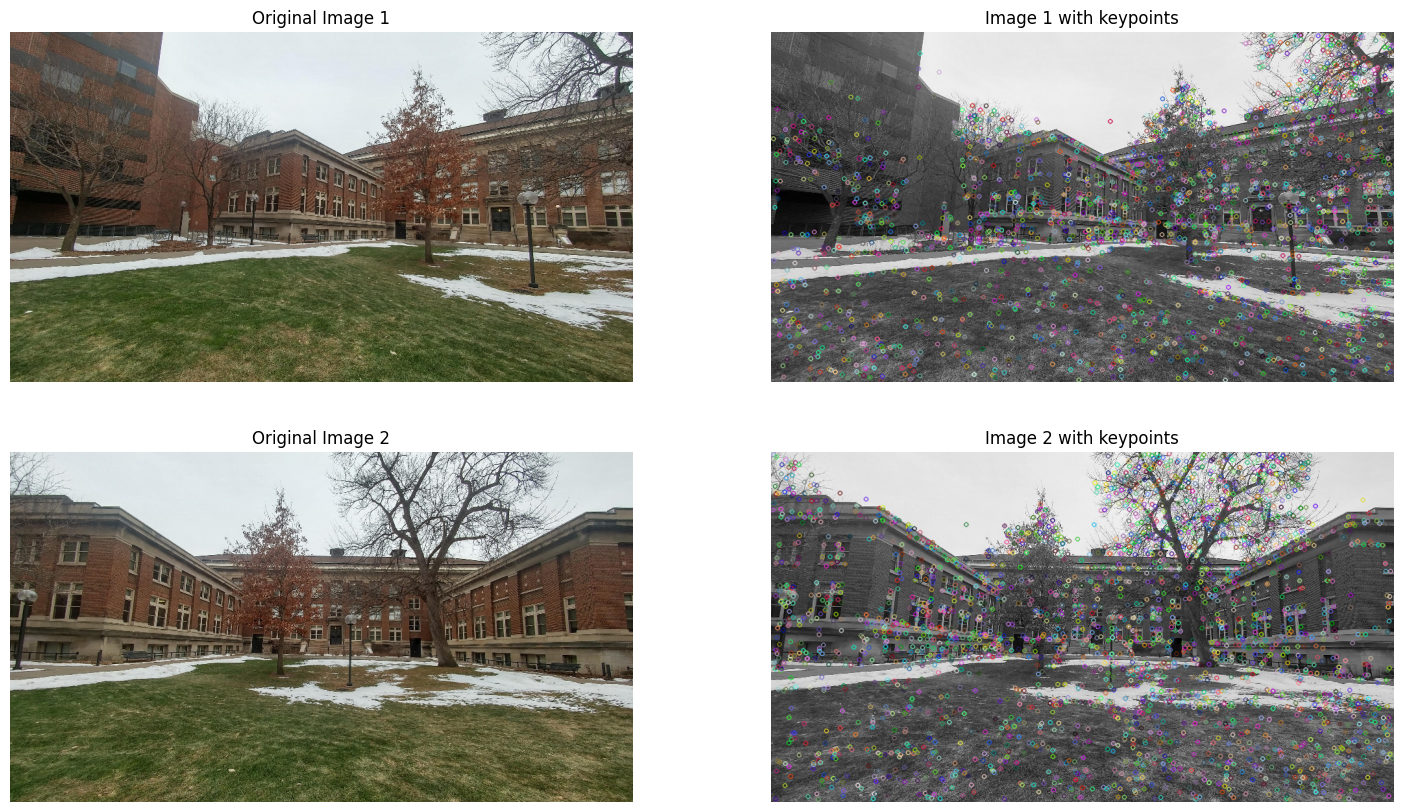
\includegraphics[width=0.675\textwidth]{Assets/keypoints.png}
        \caption{Keypoints detected in the first two images}
        \label{fig:keypoints}
    \end{figure}

    \subsection*{\textbf{Feature Matching}}
    We use the Brute-Force Matcher and the FLANN-based Matcher to match the
    keypoints in the two images. The matches are shown in Figure \ref{fig:matches}.
    We only display the matches that have a distance ratio less than $0.75$ for
    the Brute-Force Matcher and a distance ratio less than $0.7$ for the FLANN-based
    matcher. The matches are displayed on grayed images for better visibility.
    \begin{figure}[h]
        \centering
        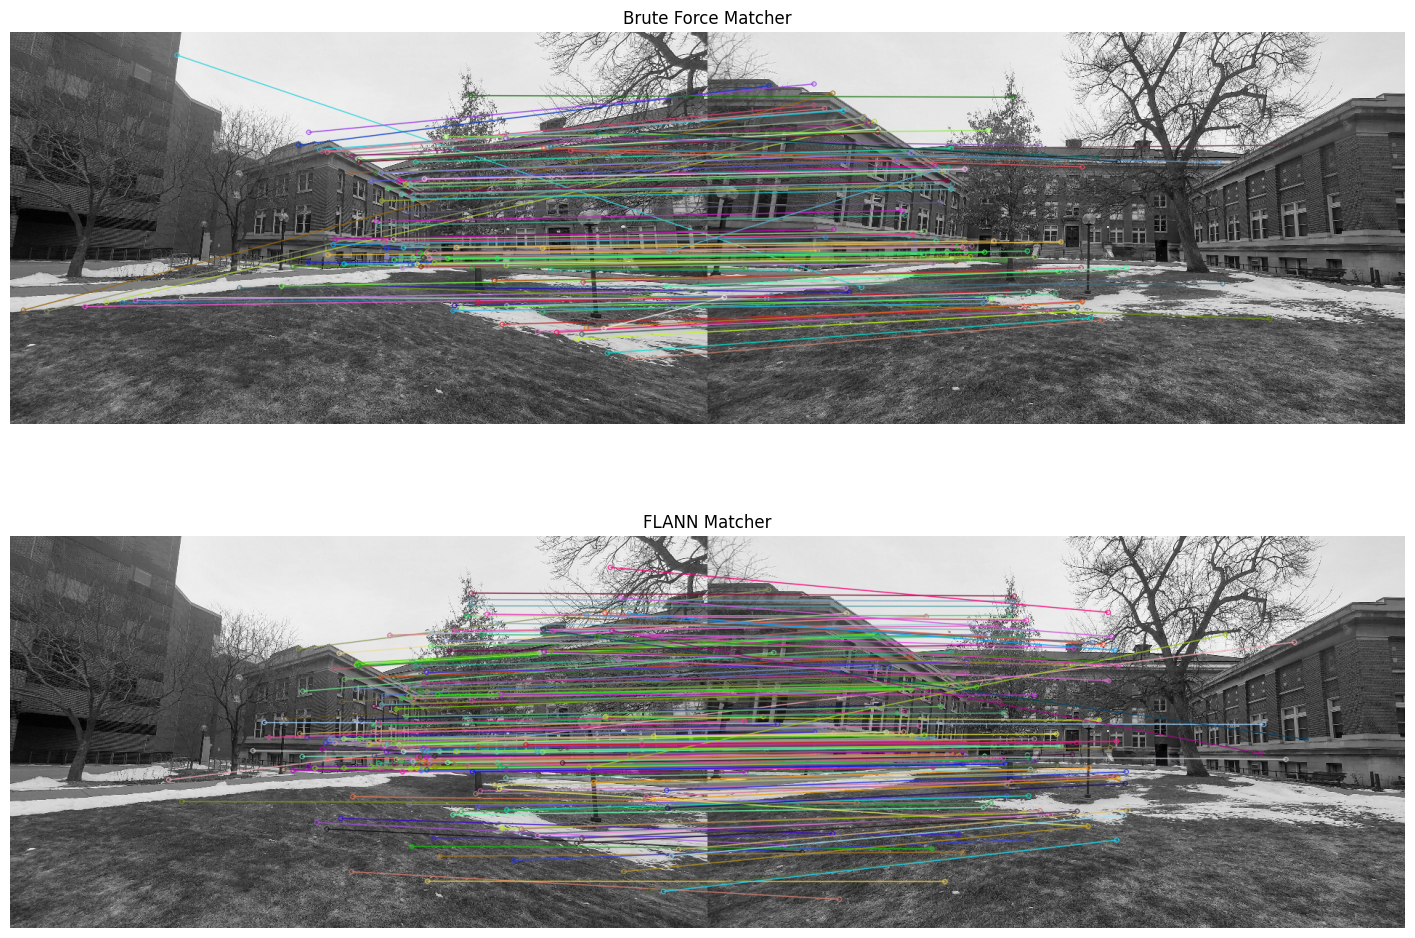
\includegraphics[width=0.85\textwidth]{Assets/matches.png}
        \caption{Matches between the keypoints in the first two images}
        \label{fig:matches}
    \end{figure}

    \subsection*{\textbf{Homography Estimation}}
    We then estimate the homography matrix using the RANSAC algorithm. The
    homography matrix is used to warp one image onto the other. The homography matrix,
    rounded up to 2 decimal places, is
    \begin{equation*}
        \mathbf{H} = \begin{bmatrix}
            -52.37 & 1.12 & 18955.0 \\
            -15.91 & -32.21 & 9880.81 \\
            -0.05 & -0.001 & 1.0
        \end{bmatrix}
    \end{equation*}

    \subsection*{\textbf{Perspective Warping}}
    We use the homography matrix to warp the second image onto the first image onto
    the viewpoint of the second image. We warp the first image to look like it was
    taken from the viewpoint of the second image. The left and right side of the image
    is shown in Figure \ref{fig:warped}.
    \begin{figure}[h]
        \centering
        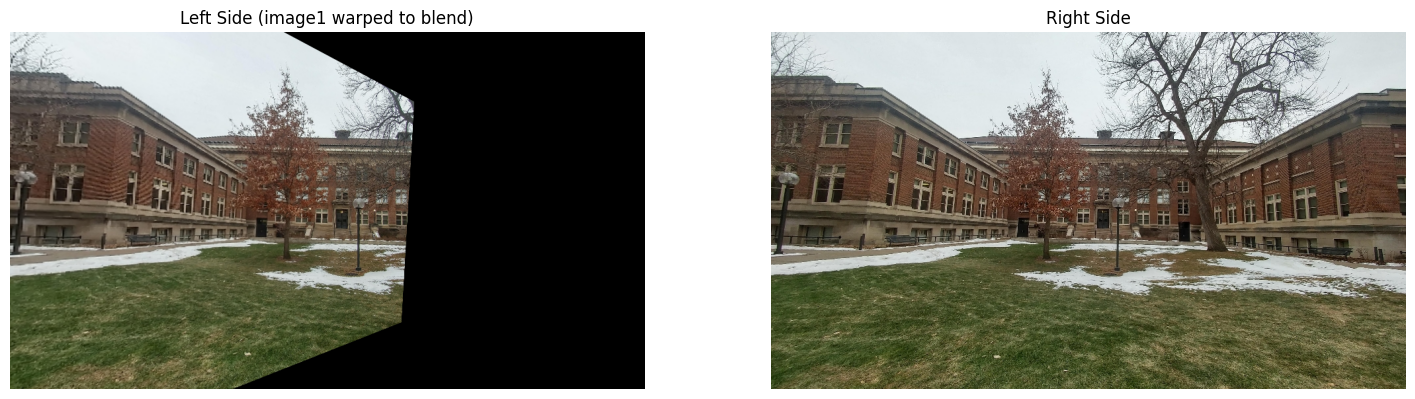
\includegraphics[width=0.85\textwidth]{Assets/warped.png}
        \caption{Warped image of the first image to the viewpoint of the second image}
        \label{fig:warped}
    \end{figure}

    \subsection*{\textbf{Stitching}}
    We next create a panorama by stitching together the warped image and the second
    image. Figure \ref{fig:panorama-unprocessed} shows the generated panorama without
    any cropping or blending.
    \begin{figure}[h]
        \centering
        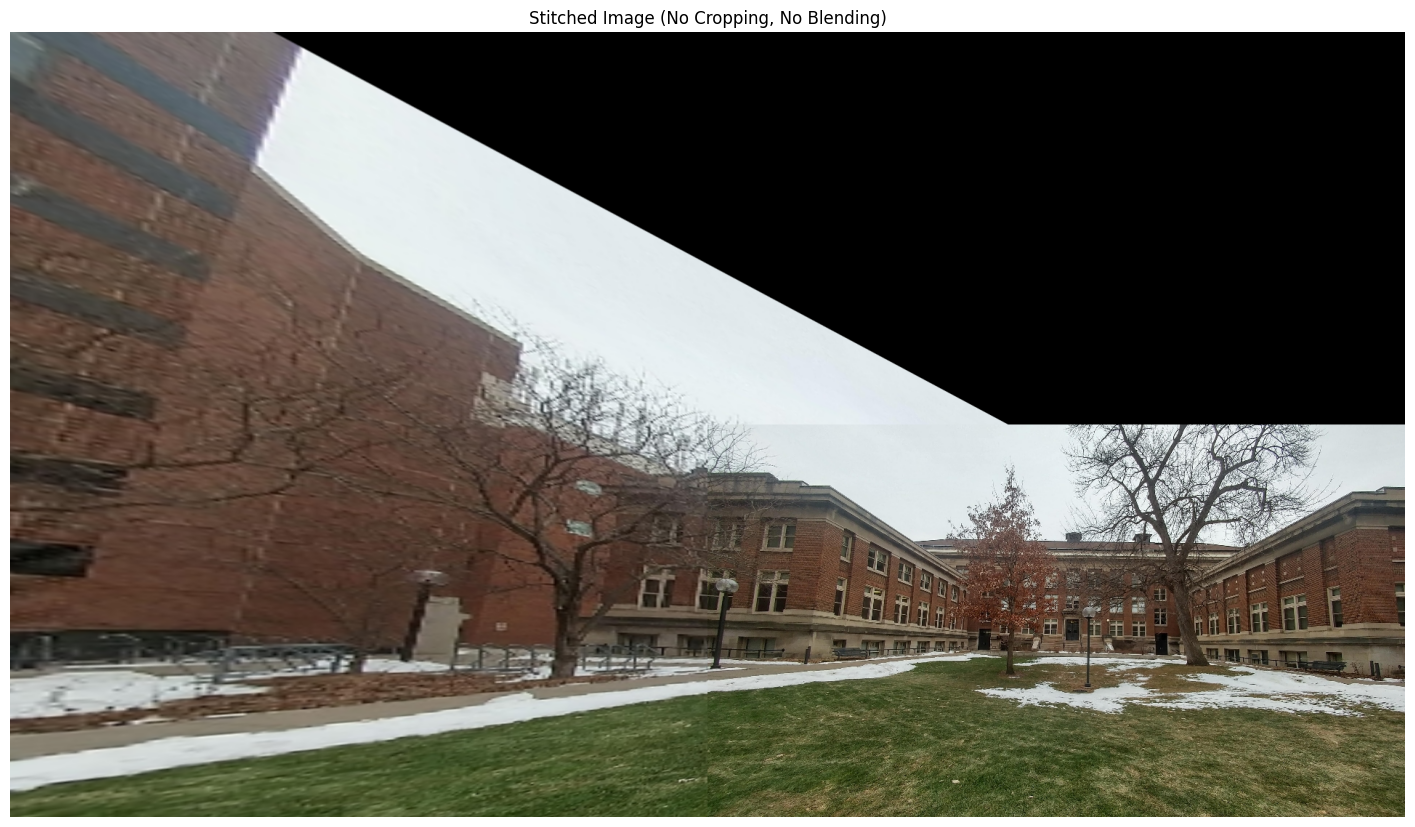
\includegraphics[width=0.815\textwidth]{Assets/panorama-unprocessed.png}
        \caption{Panorama generated without any cropping or blending}
        \label{fig:panorama-unprocessed}
    \end{figure}
    \vspace*{0pt} \\
    Figure \ref{fig:panorama-processed} shows the final panorama after cropping and
    blending the images.
    \begin{figure}[h]
        \centering
        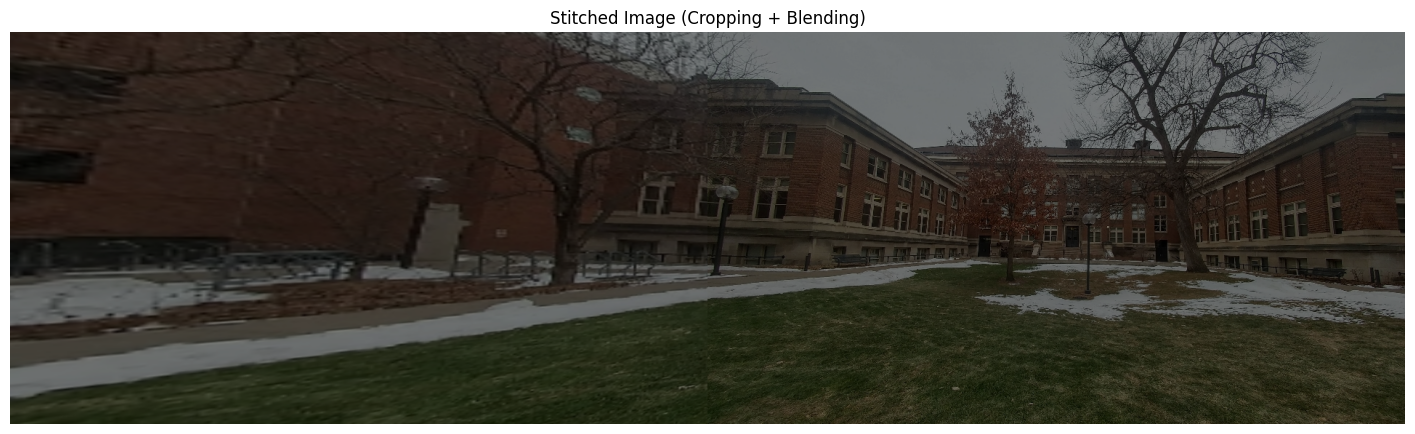
\includegraphics[width=0.815\textwidth]{Assets/panorama-processed.png}
        \caption{Final panorama after cropping and blending}
        \label{fig:panorama-processed}
    \end{figure}

    \subsection*{\textbf{Multi-Stitching}}
    Finally, we perform multi-stitching using \texttt{cv2.Stitcher()} and stitch all
    8 images into a single panorama. Figure \ref{fig:multi-stitching} shows the
    final panorama after multi-stitching.
    \begin{figure}[h]
        \centering
        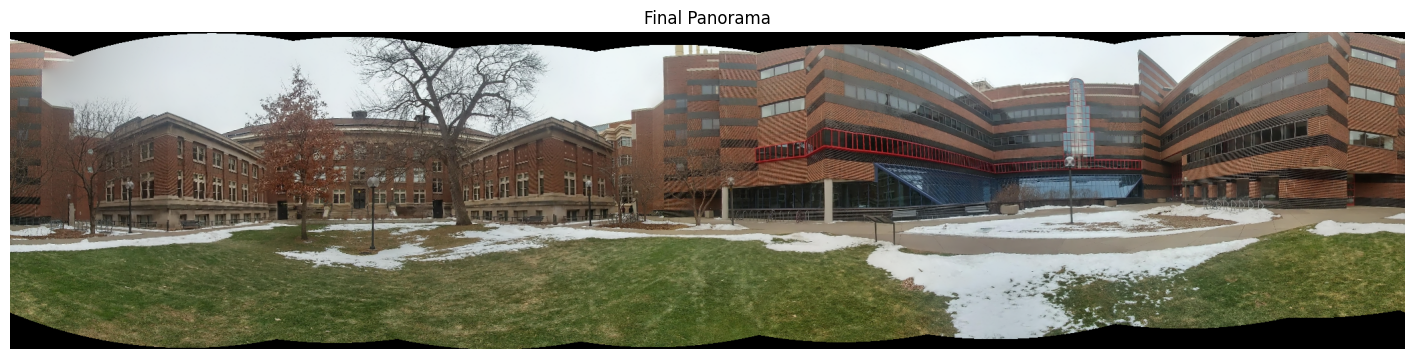
\includegraphics[width=0.815\textwidth]{Assets/multi-stitching.png}
        \caption{Final panorama after multi-stitching}
        \label{fig:multi-stitching}
    \end{figure}

    \section*{\textbf{Referneces}}
    \begin{enumerate}
        \item \href{https://inst.eecs.berkeley.edu/~ee290t/fa19/lectures/lecture10-3-decomposing-
        F-matrix-into-Rotation-and-Translation.pdf}{\textit{Lecture 10} in EE290T (Fall 2019) -
        Advanced topics in Signal Processing: 3D Image Processing \& Computer Vision, University of
        California, Berkeley}
    \end{enumerate}

\end{document}